\documentclass[../main.tex]{subfiles}

\begin{document}

\chapter{Overview of potential solutions}
\label{chap:overview}

This chapter theoretically elaborates on different approaches to implementing the requirements defined in chapter \ref{chap:requirements}.
The sketched protocols illustrate different encryption techniques.
Each section discusses the consequences of the technique to the requirements of this thesis.
The outcome of this chapter is a set of possible solution strategies.
Section~\ref{sec:modern-e2ee} relates them to modern protocols used in end-to-end encrypted applications. 
Finally, section~\ref{sec:justification} justifies why hybrid encryption is chosen as encryption technique in this thesis.

The following table summarizes the major results of this chapter.
It provides an overview for the reader.
A check (\checkmark) indicates that an approach satisfies the corresponding requirement.
A missing check means that the approach conflicts with the requirement.
Details and justifications can be found in the corresponding sections below.


\begin{table}[h]
    \centering 
    \begin{tabular}{|l|l|c|c|c|c|c|c|c|c|c|c|}
    \hline
    Section                         & Approach                  & F1          & F2          & F3            & S1            & S2            & S3            & N1            & N2            & N3            & N4            \\ \hline
    \ref{sec:external-encryption}   & External encryption       & \checkmark  & \checkmark  &               &               & \checkmark    & \checkmark    & \checkmark    & \checkmark    &               & \checkmark    \\ \hline
    \ref{sec:mutual-encryption}     & Mutual encryption         & \checkmark  & \checkmark  & \checkmark    & \checkmark    & \checkmark    & \checkmark    & \checkmark    & \checkmark    & \checkmark    &               \\ \hline
    \ref{sec:hybrid-encryption}     & Hybrid encryption         & \checkmark  & \checkmark  & \checkmark    & \checkmark    & \checkmark    & \checkmark    & \checkmark    & \checkmark    & \checkmark    & $\sim$        \\ \hline
    \ref{sec:key-server}            & Key server                & \checkmark  & \checkmark  & \checkmark    &               & \checkmark    & \checkmark    &               & \checkmark    & \checkmark    & \checkmark    \\ \hline
    \ref{sec:attribute-encryption}  & ABE                       & \checkmark  & \checkmark  & \checkmark    &               & \checkmark    & \checkmark    &               &               & \checkmark    & \checkmark    \\ \hline
    \ref{sec:broadcast-identity}    & IBBE                      & \checkmark  & \checkmark  & \checkmark    &               & \checkmark    & \checkmark    &               &               & \checkmark    & \checkmark    \\ \hline
    \ref{sec:broadcast-identity}    & CBBE                      & \checkmark  & \checkmark  & \checkmark    & \checkmark    & \checkmark    & \checkmark    & \checkmark    &               & \checkmark    & \checkmark    \\ \hline
    \ref{sec:broadcast-proxy}       & PRE                       & \checkmark  & \checkmark  & \checkmark    &               & \checkmark    & \checkmark    &               &               & \checkmark    & \checkmark    \\ \hline
\end{tabular}
\caption[Overview encryption techniques]{Overview of the considered encryption techniques and their implications to the system requirements.}
\label{tab:overview-summary}
\end{table}

\section{External encryption}
\label{sec:external-encryption}
An intuitive way of implementing a protocol that allows the exchange of encrypted logs among users is to rely on external tools.
Suppose that Alice wants to share a log with Bob.
Alice could send the log to Bob with an encrypted email.
Emails can be encrypted with standardized protocols, e.g. PGP\footnote{Defined by IETF in \href{https://www.rfc-editor.org/rfc/rfc4880}{RFC4800}.} or S/MIME\footnote{Defined by IETF in \href{https://www.rfc-editor.org/rfc/rfc8551.html}{RFC8551}.}.
They allow Alice to confidentially share logs with others.
This approach, however, is limited and does not satisfy the identified requirements.
It is the responsibility of the user to correctly apply the protocol.
This is error-prone, it could lead to unintended security issues and it is not user-friendly.
Sharing the log with $n$ users requires Alice to send $n$ encrypted emails.
More importantly, this approach does not end-to-end encrypt logs because the server storing the logs still has access to the unencrypted data.
Since the Overseer server is not trusted, confidentiality is broken (security requirement S1).
Once an encrypted email is sent to the receiver, there is no way for Alice to revoke any access to the log.
She loses control over the encrypted log because Bob's email provider stores the cipher.
This is not in the control of the toolchain.
It implies, that Alice can not revoke the access to the log anymore (functional requirement F3).
Those limitations motivate the implementation of a more sophisticated protocol.

\section{Mutual encryption}
\label{sec:mutual-encryption}
The term mutual encryption refers to the idea that logs are encrypted mutually between users in the system.
If each user is assigned a key pair, a data owner can encrypt a log for each user separately.
The core idea is similar to the approach presented for external encryption (section \ref{sec:external-encryption}).
However, this approach integrates the encryption and decryption of logs into the toolchain.
To better understand it consider the following example.
A monitor component accesses data of Alice and therefore creates a log.
Since Alice needs to be able to access the log, the monitor encrypts the log under the public key of Alice and sends it to the server.
If Alice keeps her private key secret she is the only entity who can decrypt the log.
She can download the log, decrypt it, and also share it with Bob by re-encrypting it under his public key.
The re-encrypted data is then sent to the server where it is stored.
Bob can finally download and decrypt the shared log.

All functional requirements are fulfilled:
Alice can access the log because the monitor encrypted it with her public key.
She can also share logs with others.
The encrypted data is stored by the Overseer server.
This allows Alice to request the deletion of the cipher from the server.
Thus, Alice can revoke access to the log.
As long as all users have exclusive access to their private keys, this approach also ensures the confidentiality of the log (security requirement S1).

To defend against malicious data owners creating forged logs, the monitor component (e.g. the entity creating a log) needs to cryptographically sign the log before encryption.
If Alice shares the log, she does not share the plain log.
Rather, she encrypts the signed log.
Alice can not modify the existing log or create a completely new log because she is not able to compute a valid signature in the name of the monitor.
She could only succeed by knowing the private key of the monitor.
This structure allows the receiver to verify if the log was created by a valid monitor component.
As a consequence, a forged log can be detected during decryption (security requirement S3).

Security requirement S2 can also be satisfied.
To achieve this, Alice does not only encrypt the signed log directly.
She additionally signs and includes the identity of the receiving user.
This allows receivers to verify if the log was intentionally shared with them~\cite{Davis2001}.
Figure \ref{fig:mutual_encryption} shows the structure of a shared log before it is encrypted.
The actual log data is signed by the monitor.
The shared log is a data structure that contains the signed log.
It additionally specifies the user with whom the log is shared (e.g. the receiver).
The shared log itself is signed by the data owner.
The shared log is passed to the encryption algorithm.
After a successful decryption, a receiver receives this shared log.
This allows him to validate if the sender intentionally shared the log.
The receiver can also verify if the nested access log was signed by the claimed monitor.

\begin{figure}[ht]
    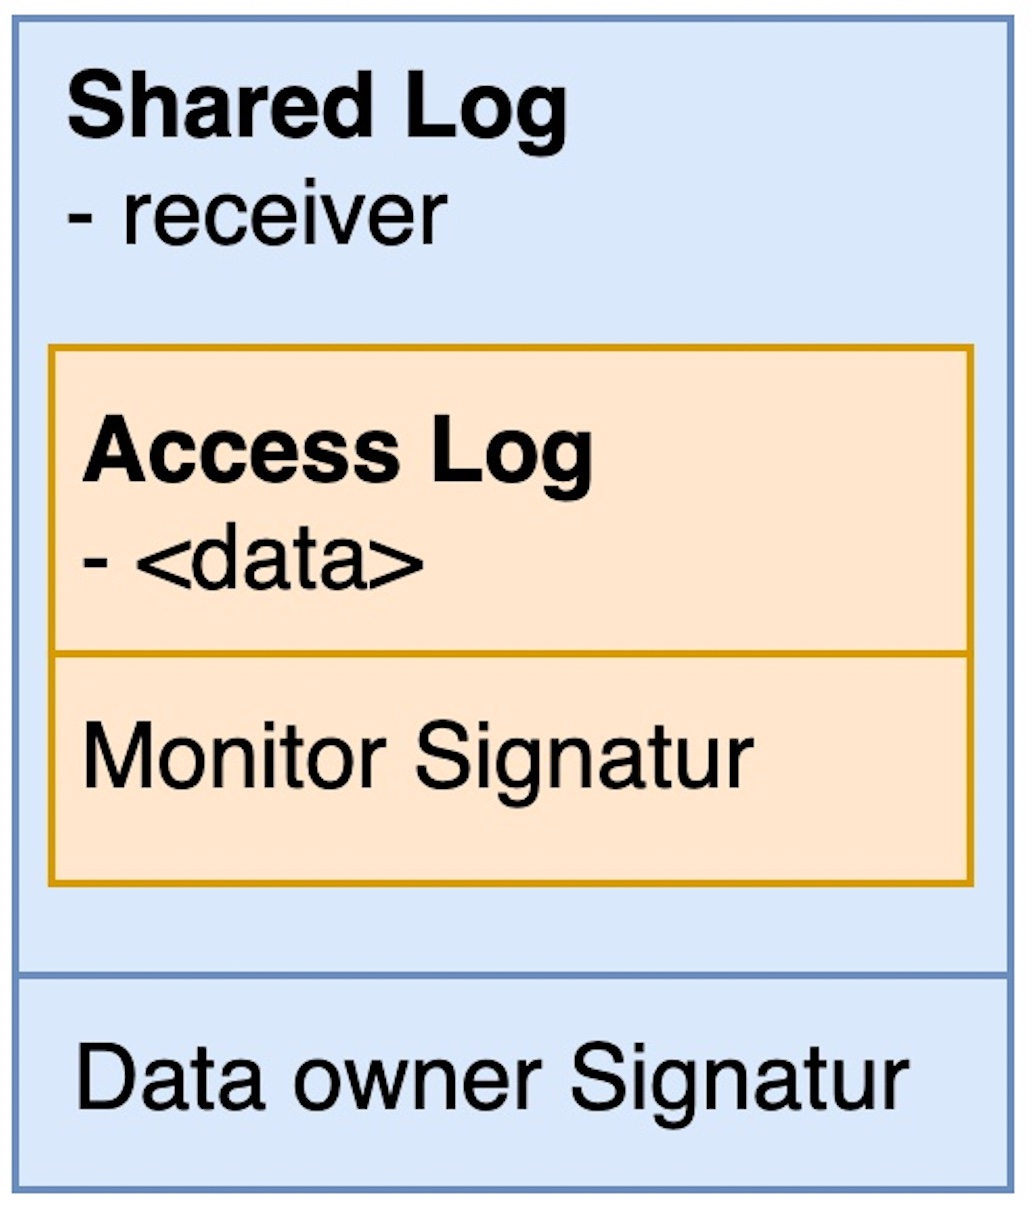
\includegraphics[scale=0.2]{../img/04/mutual_encryption.jpg}
    \centering
    \caption[Structure shared log]{Structure of a shared log before encryption.}
    \label{fig:mutual_encryption}
\end{figure}

This approach relies on standardized asymmetric cryptography (e.g. RSA).
While it fulfills all functional and security requirements it suffers from performance problems.
Similar to external encryption, the whole log needs to be encrypted $n$ times if it is shared with $n$ users.
Much more problematic, however, is the application of asymmetric cryptography to application data.
Public-key cryptography relies on intense mathematical computations and should not be used to encrypt large amounts of data directly~\cite[340]{Eckert2018}.
Eckert justifies this with the fact that asymmetric encryption algorithms are muss less performant than symmetric algorithms.
Following her argumentation, asymmetric cryptography is therefore usually used to encrypt a symmetric key which finally encrypts the larger payload with a symmetric scheme.
Thus, the implemented protocol should avoid the encryption of log data with asymmetric algorithms.

\section{Hybrid encryption}
\label{sec:hybrid-encryption}

The approach extends the concept introduced in the previous section \ref{sec:mutual-encryption}.
Hybrid encryption combines the advantages of asymmetric cryptography with the advantages of symmetric cryptography.
In a hybrid scheme, the content is encrypted via symmetric encryption.
The short symmetric key (e.g. 128 or 256 bit for AES) is then encrypted with asymmetric algorithms.
Thus, the expensive asymmetric algorithms only encrypt small amounts of data.
It is used to securely transport the symmetric key.
The larger payload is encrypted with an efficient symmetric scheme.
~\cite[340]{Eckert2018}

Consider the scenario where Alice wants to share data with Bob.
Alice initially generates a symmetric key $k$.
She uses $k$ to encrypt the payload with a symmetric scheme (e.g. AES).
She then encrypts $k$ under the public key of Bob.
Finally, she sends the encrypted key along with the encrypted payload.
To decrypt the payload, Bob first decrypts the symmetric key $k$ using his private key.
In the final step, Bob can use $k$ to decrypt the symmetrically encrypted cipher.

This concept can be applied to the context of this thesis.
An initially created log is encrypted for Alice using hybrid encryption.
This results in a ciphertext that consists of the encrypted symmetric key and the encrypted log.
The encrypted key can be decrypted only by Alice.
Alice can use the key to decrypt the log.
If she wants to share the log with Bob, she applies hybrid encryption again:
She generates a fresh symmetric key and encrypts it under Bob's public key.
The log is encrypted with the fresh key.
The encrypted key and the encrypted log are sent to the server.
This allows Bob to decrypt the log.
Additionally, Alice can specify multiple receivers by attaching multiple encrypted keys to the encrypted log -- one for each receiver.
This is visualized in figure \ref{fig:hybrid_encryption}. 
The key $k$ is used to encrypt the log in a symmetric scheme.
To make the key available to Bob and Charlie the key is encrypted for both of them using asymmetric encryption.
Alice can also revoke access to the log by re-encrypting the log. 
This requires a fresh symmetric key $k$.

\begin{figure}[ht]
    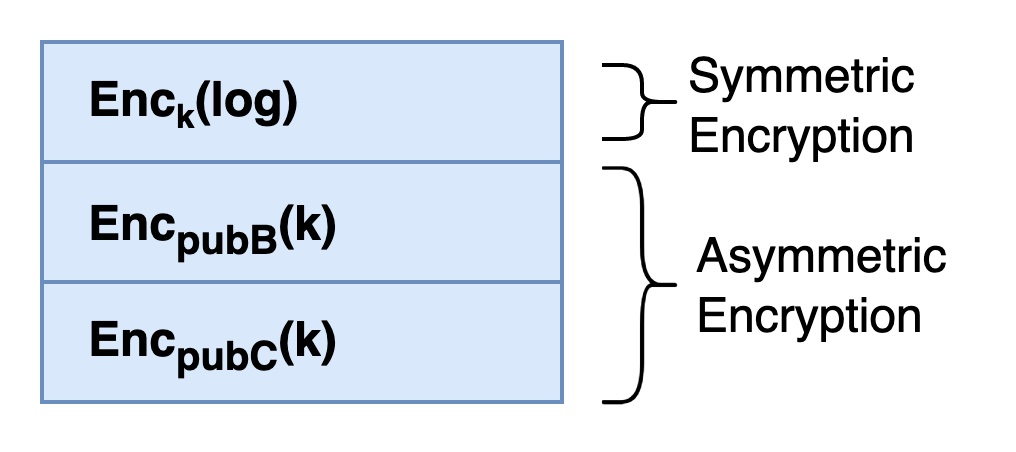
\includegraphics[scale=0.22]{../img/04/hybrid_encryption.jpg}
    \centering
    \caption[Structure encrypted log]{Structure of an encrypted log using hybrid encryption. The cipher contains the encrypted log and an encrypted key for each recipient.}
    \label{fig:hybrid_encryption}
\end{figure}

The above description shows, that hybrid encryption techniques can be used to satisfy all functional requirements.
Moreover, only those can decrypt which were explicitly specified during encryption.
This ensures that only authorized users can decrypt (security requirement S1).
To adhere to security requirements S2 and S3 the techniques introduced in section \ref{sec:mutual-encryption} can be applied with a little modification.
Instead of a single receiver, the shared log needs to contain the list of authorized users.
The shared log is finally encrypted with the symmetric key.
This allows receivers to validate if the log was intended for them and to verify if the actual log was modified during transit.
Additionally, standardized algorithms exist for symmetric and asymmetric cryptography.
This allows the construction of a secure and portable crypto library.

While this approach improves the performance compared to section \ref{sec:mutual-encryption}, there is still a drawback.
If the log is encrypted for $n$ users, the symmetric key needs to be encrypted $n$ times.

\section{Key server}
\label{sec:key-server}

The development of cloud computing and centralized software architectures motivated the idea of key servers~\cite{Seitz2003}.
A key server stores cryptographic keys on behalf of the user.
If a user authenticates against the server and has the required permissions it can access a particular key.
This can be useful in environments where multiple users need to access the same key.
The creator and owner of a key can upload the key to the key server.
If others require access to the key, the owner can modify the access policy.

The concept of a key server can also be applied to share encrypted logs.
Once a monitor creates a log because it accesses sensitive data of Alice, the monitor creates a symmetric key and encrypts the log under this symmetric key.
The encrypted log is sent to the Overseer.
To decrypt the log, Alice requires access to this symmetric key.
Thus, the monitor needs to upload the generated key to the key server which allows Alice to download it.
If she wants to share the log with Bob, there is no need to re-encrypt any data in the Overseer.
Rather, she needs to tell the key server that Bob is allowed to access this key.
Alice can also revoke access to the file by telling the key server that a particular user is not allowed to access the key anymore.
However, if a malicious user stored the key on his local machine, the revocation does not have any effect.
The encrypted log in the Overseer should therefore be re-encrypted with a freshly generated key.
This new key is then also uploaded to the key server.

This example shows that all functional requirements can be satisfied when utilizing a key server.
It can be implemented using standardized symmetric encryption schemes (e.g. AES).
The techniques introduced in section \ref{sec:mutual-encryption} to satisfy security requirements S2 (the receiver can verify it is a valid encryption endpoint) and S3 (the data owner can not forge logs) can be applied again.
Security requirement S1, however, can not be met because the system suffers from key escrow (the administrator of the key server has access to all keys).
The confidentiality of all logs is broken because this allows him to potentially decrypt all logs.
The utilization of a key server also implies that we require an additional trusted component.
This increases the attack surface of the system and does not adhere to the non-functional requirement N1 (minimal number of trusted entities).

\section{Attribute-based encryption}
\label{sec:attribute-encryption}
Data access control mechanisms validate if a user is authorized to perform an action on certain data~\cite[242]{Eckert2018}.
Access control is usually enforced by a server.
Whenever a user requests the access to data, the server checks if the user has the required permissions (e.g. if the user is employed by a specific company).
A compromised server, however, can cause serious harm to a system because the server has unlimited access to all data stored in the server~\cite{Hagg2022}.
Specifically, if data is not end-to-end encrypted an attacker can access the data in plaintext.
Attribute-based encryption mitigates that threat.
It shifts the logic of access control into the domain of cryptography~\cite{Bethencourt2007}.
Data is encrypted along with permissions.
A user can only decrypt the data if it owns the demanded permissions.

Attribute-based encryption distinguishes between attributes and policies.
Attributes (e.g. ${A,B,C}$) are assigned to users.
This assignment is encoded into a private key.
Thus, the private key of the user contains attributes which are used to check if the user has certain permissions.
Attributes can be used to create policies (e.g. $A \land B \land \neg C$).
A policy is a logical expression over attributes.
While encrypting data, the user specifies a policy which is encoded into the cipher.
A successful decryption requires a private key which satisfies the policy.

\emph{ABE} can be used directly to encrypt data for multiple receivers~\cite{Bethencourt2007}. 
During encryption, a policy is defined. 
All users which are equipped with attributes fulfilling this policy can decrypt data.
By encoding the name of the valid receivers into the policy, the encrypting user could specify the set of users who can decrypt.
If the access of a user needs to be revoked, the cipher is re-encrypted with a new set of receivers.
This ensures that all required functional requirements are met.
One can again equip the logs with cryptographic signatures (as described in section \ref{sec:mutual-encryption}).
Those techniques fulfill the security requirements S2 (the receiver can verify it is a valid encryption endpoint) and S3 (the data owner can not forge logs).

Attribute-based encryption usually relies on a trusted key generation center~\cite{Sahai2009}.
It computes and distributes cryptographic keys.
This implies key escrow and harms security requirement S1 because the trusted server can potentially decrypt all ciphers.
Additionally, each trusted entity increases the attack surface of the toolchain and conflicts with the non-functional requirement N1 (minimal number of trusted entities).
There are also schemes that avoid a centralized trust center by employing a decentralized architecture~\cite{Vaanchig2018}.
These systems, however, can not be integrated into the centralized architecture of the existing toolchain.
A lot of papers are published in the field of attribute-based encryption.
However, no cryptographic standard exists conflicting with the non-functional requirement N2.
It is not included in the Web Cryptographic API~\cite{WebCryptoApi2017}.

\section{Broadcast encryption}
\label{sec:broadcast-encryption}

Broadcast encryption (\emph{BE}) is an encryption technique that allows the encrypting user to specify a set of authorized recipients.
Only those users can decrypt the produced ciphertext.
It was initially proposed by~\citeauthor{fiat1993broadcast}~\cite{fiat1993broadcast}.
In the last years different realization of broadcast encryption schemes were discussed~\cite{Sakai2007, Li2018, Hagg2022, Fan2013}.
This section categorizes and summarizes those approaches as suggested in~\cite{Hagg2022}.
Furthermore, each approach is evaluated against the system requirements.

\subsection{Identity-based broadcast encryption} 
\label{sec:broadcast-identity}

Traditional identity-based encryption (\emph{IBE})) schemes are  a type of public-key cryptography.
The public key of a user is a human rememberable string (e.g. the email address).
For a given public key the private key can be generated using a dedicated derivation function.
Those private keys must be computed by a trusted entity which has access to secret system parameters.~\cite{shamir1985}

This basic idea was later adopted to implement broadcast encryption~\cite{Hagg2022}.
The resulting schemes are called identity-based broadcast encryption (\emph{IBBE})~\cite{Sakai2007}.
The following example illustrates its functionality~\cite{Hagg2022}:
Assume the users Alice and Bob.
Both own unique email addresses.
First of all, the \emph{IBBE} scheme needs to be instantiated.
The trust center computes the private keys on behalf of Alice and Bob based on their email addresses.
It also distributes the private keys and public system parameters to both users.
Alice wants to send confidential data to Bob.
She applies the encryption algorithm which requires a set of public keys and the public system parameters as input.
Next, she uploads the cipher to a server.
This allows Bob to download and decrypt it using his private key.
In order to revoke a user, Alice must re-encrypt the data and upload it again.

The example shows that all three functional requirements can be fulfilled.
The techniques from section \ref{sec:mutual-encryption} can be applied again.
This satisfies the security requirement S2 (the receiver can verify it is a valid encryption endpoint) and S3 (the data owner can not forge logs).
\emph{IBBE} schemes suffer from key escrow because a trusted party computes and distributes private keys~\cite{Hagg2022}.
This breaks the confidentiality of the encrypted logs (security requirement S2).
The additional trusted entity also increases the attack surface breaking non-functional requirement N1 (minimal number of trusted entities).
A lot of research is going on in the field of \emph{IBE}~\cite{Hagg2022}.
However, no cryptographic standard exists for \emph{IBE} or \emph{IBBE}.
It is not included in the Web Cryptographic API~\cite{WebCryptoApi2017}.
This conflicts with the non-functional requirement N3.

\subsection{Certificate-based broadcast encryption}
\label{sec:broadcast-certificate}

Certificate-based encryption (\emph{CBE}) was initially proposed in 2003~\cite{Gentry2003}. 
The following observations motivated this approach~\cite{Hagg2022}:
\begin{itemize}
    \item 
    Traditional public key encryption schemes are faced with the certificate revocation problem (details in \cref{terms}).
    \item 
    Identity-based encryption schemes usually rely on trusted entities. 
    This introduces key escrow (details in \cref{IBBE}).
    However, they do not suffer from the certificate revocation problem.
    \item 
    Traditional public key schemes can be combined with identity-based schemes by double encrypting the plaintext.
    In particular, the plaintext is encrypted once under the public key of the traditional scheme and once under the public key of the identity-based scheme.
    The result of this construction are \emph{CBE} schemes.
    They eliminate key escrow and the certificate revocation problem.
\end{itemize}

This idea was later adopted to broadcast encryption yielding a certificate-based broadcast encryption scheme (\emph{CBBE})~\cite{Li2018}.
Although this construction relies on a key generation center, it does not suffer from key escrow~\cite{Hagg2022}.
Once keys are established, a user can encrypt data for dedicated recipients.
Only the users specified during encryption can decrypt the cipher.
The key generation center can not decrypt the cipher because it does not have access to any private key of the traditional scheme~\cite{Hagg2022}.
Besides the functional requirements, \emph{CBBE} also satisfies the security requirements.
The distinction of shared log and signed log introduced in section \ref{sec:mutual-encryption} can be applied again.
Thus, all receivers can validate that they are intended decryption endpoints (security requirement S2) and that the access log was created by the claimed monitor (security requirement S3).
The notion of E2EE is also fulfilled because the trusted server can not decrypt the logs.

Unfortunately, no reference implementations of \emph{CBBE} exist.
This fact is a major drawback in the context of this thesis.
These cryptographic systems are currently the subject of research.
There are no ongoing standardization processes to analyze their security.
As a result, the non-functional requirement N2 (standardized cryptographic algorithms) can not be met.
Using those schemes in a practical implementation is avoided in this thesis because the missing standards introduce an unpredictable risk.

\subsection{Proxy re-encryption based broadcast encryption}
\label{sec:broadcast-proxy}
Proxy re-encryption (\emph{PRE}) is another encryption technique proposed to realize broadcast encryption~\cite{Hagg2022}.
Its fundamental concept relies on a trusted proxy which can transform encrypted data between users.
It is an important requirement of those schemes that the proxy does not learn anything about the plaintext during this re-encryption~\cite{Chen2018}.

Similar to the example given in~\cite{Hagg2022}, consider a user Alice who stores a ciphertext $E_A$ in the cloud.
Only Alice can decrypt $E_A$, however, she wants to make the plaintext available for Bob.
This requires Alice to share a re-encryption key $rk_{Alice,Bob}$ with the proxy.
The knowledge of this key allows the proxy to transform $E_A$ to $E_B$.
Bob can then download and decrypt $E_B$
Alice could revoke access to a log by instructing the server to delete the cipher for a dedicated user.

The proxy needs to be semi-trusted because with the knowledge of $rk_{Alice,Bob}$ it can re-encrypt all ciphers from Alice to Bob~\cite{Chen2018}.
This has important consequences for the security of the protocol implemented in this thesis.
Once Alice defined Bob as a valid receiver for a single log, the server could re-encrypt all ciphers of Alice for Bob.
This, however, affects the confidentiality of encrypted logs.
Not only authorized users might have access.
Users might collude with the server (which re-encrypts logs on behalf of the user) to obtain decrypted logs.
Overall, a proxy re-encryption based scheme does not adhere security requirement S1 (confidentiality of logs).
Notice that no cryptographic standard exists for proxy re-encryption based cryptography.
It is not included in the Web Cryptographic API~\cite{WebCryptoApi2017}.
This conflicts with the non-functional requirement N3.

\section{E2EE in modern technology}
\label{sec:modern-e2ee}

Many modern communication applications rely on E2EE. 
This section exemplarily investigates the implemented protocols of Zoom, CloudSeal and of the messaging services Whatsapp and Signal.
The goal of this section is to demonstrate what E2EE techniques are practically used in modern applications.
Moreover, those approaches are discussed in the context of the this thesis.
All following techniques have in common that they do not rely on a PKI.
This restriction, however, is not necessary for this thesis because the inverse transparency toolchain is intended to be distributed in an enterprise context.
This simplifies the design of the final protocol.

\subsection{Zoom}
Zoom provides a video conference platform\footnote{\url{https://zoom.us/}}. 
It has integrated E2EE in their application to protect the communication among participants.
The enterprise claims that even the Zoom service provider can not decrypt the exchanged data.~\cite{Blum2020}

Once a meeting is started, the initiator of the meeting generates a meeting key.
This secret is shared among all users participating in the meeting.
Thus, the key needs to be transported securely to all users joining the meeting.
In particular, this requires the joining users to be online.
All communication is encrypted using the shared meeting key and a symmetric encryption schemes (AES-GCM).
~\cite{Isobe2021}

The protocol of Zoom is similar to the hybrid encryption described in section \ref{sec:hybrid-encryption}.
However, it can not be applied in the context of this thesis because all participating users must be online.
This assumption does not hold in the context of the inverse transparency toolchain.
Specifically, a monitor needs to be able to encrypt a log for the data owner even the data owner is offline.
The approach of Zoom shows, however, that hybrid encryption is practically used to broadcast encrypted data to multiple receivers.

\subsection{CloudSeal}
CloudSeal~\cite{Xiong2012} is a scheme to securely share and distribute files over cloud-based storages (e.g. AmazonS3).
Their E2EE relies on proxy re-encryption based encryption (see section~\ref{sec:broadcast-proxy} for details).
CloudSeal can currently not be provided as a web application because it relies on advanced cryptographic algorithms which are not included in the Wep Cryptographic API.
Thus, their clients are required to run on native operating systems.~\cite{Xiong2012}

As highlighted in section~\ref{sec:broadcast-proxy}, the construction of proxy re-encryption based schemes violates the identified requirements of this thesis.
CloudSeal is exemplarily listed here because it shows that broadcast encryption schemes are practically implemented to achieve E2EE.
It is not an option for this thesis because of the limited algorithms provided in the Wep Cryptographic API.

\subsection{Instant messaging services}
Whatsapp\footnote{\url{https://www.whatsapp.com/}} and Signal\footnote{\url{https://signal.org/}} are two popular instant messaging services.
They claim to implement E2EE.
Both services rely on the Signal protocol.
The Signal protocol is a combination of the X3DH protocol~\cite{Marlinspike2016} and the Double Ratched protocol~\cite{Perrin2016}.
The X3DH protocol establishes a shared secret between two authenticated users.
This effectively allows the initialization of a secure channel between the users.
The shared secret is used in the Double Ratched protocol to exchange encrypted messages.~\cite{Marlinspike2016, Perrin2016}

The architecture of the Signal protocol establishes sessions between users.
Encrypted data can be exchange within those session.
Encryption and decryption always requires the initially established shared secret.
If a hardware device is available (e.g. a smartphone with a secure storage element), this shared secret can be stored securely. 
When encrypting data for a set of users (e.g. within a group chat) the plaintext is encrypted for each user separately.~\cite{Marlinspike2014}

Unfortunately, the concept of sessions relying on an initially exchanged private key does not fit the architecture of the toolchain.
The Clotilde front-end allows users to login in a web application.
Within this application the encrypted data is downloaded and decrypted.
A session (as used in the Signal protocol) requires, however, that the exchange shared key is available for the user during decryption.
Since the user can login from arbitrary devices and browsers, the session key needs to be transported among those devices.
Either the user handles this manually (this conflicts with usability) or a trusted server stores the session key (this conflicts with the notion of E2EE).
In both ways the requirements of this thesis can not be met.
A possible solution to fix this is the implementation and distribution of the Clotilde front-end as an app.
This way, a secure session could be established among users and the shared secret could be securely stored in dedicated secure hardware storages which are not available in browsers.

\section{Justification of hybrid encryption}
\label{sec:justification}
The protocol designed in this thesis relies on hybrid encryption.
The purpose of this section is the justification of this encryption technique.
Recall table \ref{tab:overview-summary}, where different approaches were evaluated under the given requirements.
The table visualizes the fulfillment of the requirements of each considered approach.
Hybrid encryption satisfies all functional and security requirements.
Only the non-functional performance criterion N4 can not be fully met because the symmetric key needs to be encrypted for all receivers.
The following argumentation illustrates why hybrid encryption is nevertheless the most promising approach.

First of all, hybrid encryption improves mutual encryption because it avoids encrypting application data with asymmetric cryptography.
Instead of encrypting a log multiple times under different public keys, hybrid encryption applies fast symmetric algorithms to encrypt the log.
It then additionally encrypts the symmetric key under the public keys of the receivers.
This adheres to currently proposed best practices in applying cryptography~\cite[340]{Eckert2018}.
The performance difference might not be noticeable in the current protocol because the encrypted logs do not contain a lot of information.
However, the usage of hybrid encryption ensures that the encryption is still performant if the logs are extended in the future.
Notice that there is no difference in terms of security and functionality between the approaches.
Thus, hybrid encryption outperforms mutual encryption.

Another option to implement the intended protocol is based on broadcast encryption techniques that encrypt data for multiple receivers.
As elaborated in section \ref{sec:broadcast-encryption}, different approaches are proposed to implement broadcast encryption.
In general, there is no need to encrypt data $n$ times when it needs to be decrypted by $n$ users in those schemes.
Considering the non-functional criterion N4 (minimal resource utilization), broadcast encryption, therefore, outperforms hybrid encryption.
The main disadvantage of broadcast encryption is the missing standardization.
Specifically, the Web Cryptographic API does not include any of those schemes.
Thus, they can only be used in the browser if the reference implementations are translated into Javascript.
Since Javascript is an interpreted language, however, this comes with considerable performance limitations.
Moreover, the cryptographic library implemented in this thesis needs to be delivered in three programming languages.
Translating a dedicated scheme into multiple languages is complex, error-prone, and not realizable within the time constraint of this thesis.
Please also notice that each approach introduced in section \ref{sec:broadcast-encryption} additionally suffers from security limitations undermining the understanding of E2EE.
Since hybrid encryption relies on standardized and well-researched algorithms, it is preferred over broadcast encryption techniques.

A third option is an implementation based on a key server.
The log is encrypted with a symmetric scheme and access to the decryption key is maintained by a key server.
This approach only relies on well-researched symmetric encryption techniques.
It can therefore be implemented in different programming languages and environments.
A key server, however, introduces key escrow which harms the intended E2EE.
This is a major drawback compared to hybrid encryption.

\end{document}
